\documentclass[11pt,a4paper]{report}

% ============================================================================
% PACKAGES
% ============================================================================
\usepackage[utf8]{inputenc}
\usepackage[T1]{fontenc}
\usepackage{helvet}
\renewcommand{\familydefault}{\sfdefault}
\usepackage[margin=2.3cm, headheight=25pt]{geometry}
\usepackage{xcolor}
\usepackage{colortbl}
\usepackage{booktabs}
\usepackage{tabularx}
\usepackage{array}
\usepackage{graphicx}
\usepackage{tikz}
\usepackage{fancyhdr}
\usepackage{enumitem}
\usepackage{multirow}
\usepackage{calc}
\usepackage{amssymb}
\usepackage{pifont}
\usepackage{titlesec}
\usepackage{tocloft}
\usepackage[hidelinks]{hyperref}
\usepackage{float}
\usepackage{eurosym}
\usetikzlibrary{shapes.geometric, arrows, positioning, calc, patterns, shadows}

% ============================================================================
% COLOR DEFINITIONS - KBC INSPIRED PROFESSIONAL PALETTE
% ============================================================================
\definecolor{kbcblue}{RGB}{0, 51, 102}
\definecolor{kbcgreen}{RGB}{0, 128, 0}
\definecolor{miloprimary}{RGB}{25, 65, 150}
\definecolor{milosecondary}{RGB}{65, 105, 185}
\definecolor{miloaccent}{RGB}{10, 130, 180}
\definecolor{freegray}{RGB}{90, 95, 105}
\definecolor{bronzecolor}{RGB}{160, 100, 40}
\definecolor{silvercolor}{RGB}{130, 135, 145}
\definecolor{goldcolor}{RGB}{185, 145, 15}
\definecolor{platinumcolor}{RGB}{100, 70, 175}
\definecolor{successgreen}{RGB}{22, 160, 72}
\definecolor{warningorange}{RGB}{200, 100, 20}
\definecolor{dangerred}{RGB}{180, 55, 55}
\definecolor{lightbg}{RGB}{245, 248, 252}
\definecolor{darktext}{RGB}{25, 35, 55}
\definecolor{infoblue}{RGB}{40, 100, 180}
\definecolor{darkgreen}{RGB}{15, 125, 60}
\definecolor{appstoreblue}{RGB}{0, 85, 175}
\definecolor{datapurple}{RGB}{110, 70, 180}
\definecolor{analyticsteal}{RGB}{15, 140, 130}
\definecolor{competitorblue}{RGB}{50, 100, 180}
\definecolor{sourcegray}{RGB}{70, 80, 95}
\definecolor{healthgreen}{RGB}{46, 160, 67}
\definecolor{healthyellow}{RGB}{212, 175, 55}
\definecolor{healthorange}{RGB}{230, 126, 34}
\definecolor{healthred}{RGB}{192, 57, 43}

% ============================================================================
% HYPERREF SETUP
% ============================================================================
\hypersetup{
    colorlinks=true,
    linkcolor=miloprimary,
    urlcolor=miloprimary,
    pdftitle={MILO - Revolutionary Smart Budget \& Health App - KBC Start It Seed Funding},
    pdfauthor={DeepmAInd B.V.}
}

% ============================================================================
% HEADER/FOOTER CONFIGURATION
% ============================================================================
\pagestyle{fancy}
\fancyhf{}
\fancyhead[L]{\textcolor{kbcblue}{\textbf{MILO}}}
\fancyhead[R]{\textcolor{freegray}{KBC Start It | Seed Funding Application}}
\fancyfoot[C]{\textcolor{freegray}{\thepage}}
\renewcommand{\headrulewidth}{2pt}
\renewcommand{\headrule}{\hbox to\headwidth{\color{kbcblue}\leaders\hrule height \headrulewidth\hfill}}

% ============================================================================
% CHAPTER/SECTION FORMATTING
% ============================================================================
\titleformat{\chapter}[display]
{\normalfont\huge\bfseries\color{kbcblue}}
{\chaptertitlename\ \thechapter}{20pt}{\Huge}
\titlespacing*{\chapter}{0pt}{-30pt}{30pt}

\titleformat{\section}
{\normalfont\Large\bfseries\color{miloprimary}}
{\thesection}{1em}{}

\titleformat{\subsection}
{\normalfont\large\bfseries\color{milosecondary}}
{\thesubsection}{1em}{}

% ============================================================================
% TABLE OF CONTENTS FORMATTING
% ============================================================================
\renewcommand{\cftchapfont}{\bfseries\color{kbcblue}}
\renewcommand{\cftsecfont}{\color{darktext}}
\renewcommand{\cftsubsecfont}{\color{freegray}}
\renewcommand{\cftchapleader}{\cftdotfill{\cftdotsep}}

% ============================================================================
% CUSTOM COMMANDS
% ============================================================================
\newcommand{\alertbox}[3]{%
    \begin{tikzpicture}
        \node[fill=#1!12, draw=#1, line width=2pt, rounded corners=10pt,
              inner sep=18pt, text width=\textwidth-40pt, align=left,
              drop shadow={shadow xshift=2pt, shadow yshift=-2pt, opacity=0.15}] {
            \textcolor{#1}{\textbf{\large #2}}\\[10pt]
            #3
        };
    \end{tikzpicture}%
}

\newcommand{\statbox}[3]{%
    \begin{tikzpicture}
        \node[fill=#1!12, draw=#1, line width=1.5pt, rounded corners=8pt,
              minimum width=3.6cm, minimum height=2cm, align=center,
              drop shadow={shadow xshift=1pt, shadow yshift=-1pt, opacity=0.1}] {
            \textcolor{#1}{\textbf{\small #2}}\\[5pt]
            \textcolor{darktext}{\textbf{\Large #3}}
        };
    \end{tikzpicture}%
}

\newcommand{\revenuestream}[4]{%
    \begin{tikzpicture}
        \node[fill=#1!12, draw=#1, line width=2pt, rounded corners=10pt,
              minimum width=4.5cm, minimum height=2.4cm, align=center] {
            \textcolor{#1}{\textbf{\large #2}}\\[6pt]
            \textcolor{darktext}{\textbf{Y3: #3}}\\[3pt]
            \textcolor{freegray}{\small #4}
        };
    \end{tikzpicture}%
}

\newcommand{\tierbox}[5]{%
    \begin{tikzpicture}
        \node[fill=#1!12, draw=#1, line width=2pt, rounded corners=10pt,
              minimum width=3cm, minimum height=2.8cm, align=center,
              drop shadow={shadow xshift=1pt, shadow yshift=-1pt, opacity=0.1}] {
            \textcolor{#1}{\textbf{#2}}\\[5pt]
            \textcolor{darktext}{\small #3 receipts}\\[4pt]
            \textcolor{#1}{\textbf{\large #4}}\\[3pt]
            \textcolor{freegray}{\footnotesize #5}
        };
    \end{tikzpicture}%
}

\newcommand{\infobox}[2]{%
    \begin{tikzpicture}
        \node[fill=#1!10, draw=#1, line width=1.5pt, rounded corners=10pt,
              inner sep=18pt, text width=\textwidth-40pt, align=left] {#2};
    \end{tikzpicture}%
}

\newcommand{\sourcebox}[1]{%
    \begin{tikzpicture}
        \node[fill=sourcegray!8, draw=sourcegray, line width=1pt, rounded corners=5pt,
              inner sep=10pt, text width=\textwidth-35pt, align=left] {
            \textcolor{sourcegray}{\textbf{\footnotesize Source:} \footnotesize #1}
        };
    \end{tikzpicture}%
}

\newcommand{\competitorbox}[5]{%
    \begin{tikzpicture}
        \node[fill=#1!10, draw=#1, line width=1.5pt, rounded corners=10pt,
              inner sep=15pt, text width=\textwidth-40pt, align=left] {
            \textcolor{#1}{\textbf{\Large #2}}\\[10pt]
            \begin{minipage}[t]{0.55\textwidth}
                \textbf{Profile}\\[5pt]
                #3
            \end{minipage}
            \hfill
            \begin{minipage}[t]{0.40\textwidth}
                \textbf{vs MILO}\\[5pt]
                #4\\[8pt]
                \textbf{Threat:} #5
            \end{minipage}
        };
    \end{tikzpicture}%
}

\newcommand{\cmark}{\textcolor{successgreen}{\ding{51}}}
\newcommand{\xmark}{\textcolor{dangerred}{\ding{55}}}
\newcommand{\wmark}{\textcolor{warningorange}{\ding{115}}}
\newcommand{\threatlevel}[2]{\textcolor{#1}{\textbf{#2}}}

\newcommand{\healthscore}[2]{%
    \begin{tikzpicture}
        \node[fill=#1!20, draw=#1, line width=1pt, rounded corners=3pt,
              minimum width=0.6cm, minimum height=0.6cm, align=center] {
            \textcolor{#1}{\textbf{\small #2}}
        };
    \end{tikzpicture}%
}

% ============================================================================
% DOCUMENT BEGIN
% ============================================================================
\begin{document}

% ============================================================================
% TITLE PAGE
% ============================================================================
\begin{titlepage}
    \begin{tikzpicture}[remember picture, overlay]
        % Top gradient bar
        \fill[kbcblue] (current page.north west) rectangle ([yshift=-3.5cm]current page.north east);
        % Bottom accent
        \fill[milosecondary!25] (current page.south west) rectangle ([yshift=2cm]current page.south east);
        % Diagonal accent
        \fill[kbcblue!15] ([yshift=-3.5cm]current page.north west) -- ([yshift=-5cm]current page.north west) -- ([yshift=-3.5cm, xshift=8cm]current page.north west) -- cycle;
    \end{tikzpicture}

    \vspace*{0.5cm}

    \begin{center}
        % KBC Logo and Prepared for text
        {\large\textcolor{freegray}{\textit{Prepared for}}}

        \vspace{0.4cm}

        % KBC Logo
        
\includegraphics[height=2.5cm]{images/kbc-logo.png}

        \vspace{0.2cm}
        {\small\textcolor{freegray}{\textit{Start it @KBC Belgium | Seed Funding Application}}}

        \vspace{1cm}

        % MILO Logo
        
\begin{tikzpicture}
            \node[fill=white, draw=kbcblue, line width=4pt, rounded corners=18pt,
                  minimum width=6cm, minimum height=3cm, align=center,
                  drop shadow={shadow xshift=3pt, shadow yshift=-3pt, opacity=0.2}] {
                {\fontsize{50}{60}\selectfont\textcolor{kbcblue}{\textbf{MILO}}}
            };
        \end{tikzpicture}

        \vspace{0.6cm}

        {\LARGE\textcolor{milosecondary}{\textbf{Revolutionary Smart Budget, Receipt \& Health Intelligence}}}\\[0.4cm]
        {\large\textcolor{freegray}{The world's first app combining receipt scanning, AI health scoring, and spending analytics}}

        \vspace{1cm}

        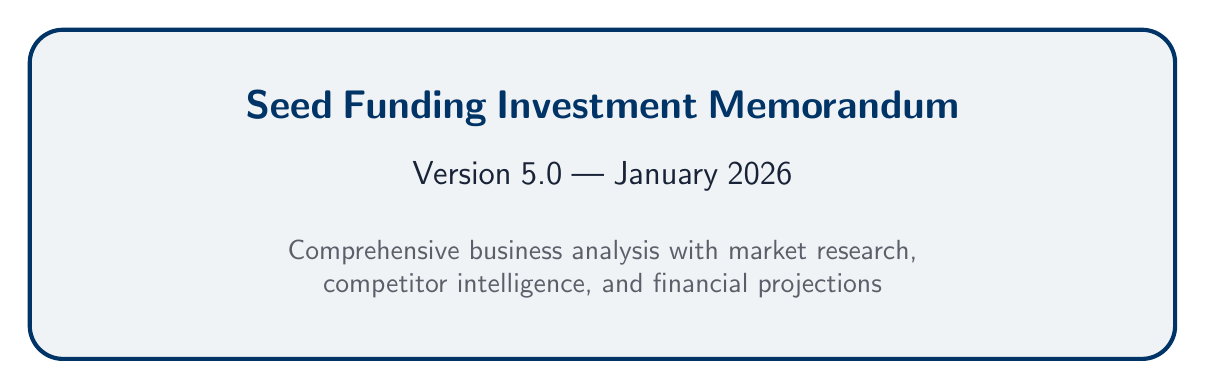
\begin{tikzpicture}
            \node[fill=kbcblue!6, draw=kbcblue, line width=1.5pt, rounded corners=12pt,
                  inner sep=22pt, text width=13cm, align=center] {
                {\Large\textcolor{kbcblue}{\textbf{Seed Funding Investment Memorandum}}}\\[12pt]
                {\large\textcolor{darktext}{Version 5.0 | January 2026}}\\[15pt]
                \textcolor{freegray}{Comprehensive business analysis with market research,}\\
                \textcolor{freegray}{competitor intelligence, and financial projections}
            };
        \end{tikzpicture}

        \vspace{1.5cm}

        % Key metrics preview
        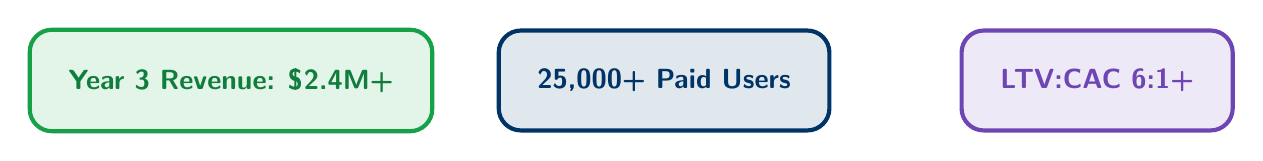
\begin{tikzpicture}
            \node[fill=successgreen!12, draw=successgreen, line width=1.5pt, rounded corners=8pt,
                  inner sep=14pt] at (0,0) {
                \textcolor{darkgreen}{\textbf{Year 3 Revenue: \$2.4M+}}
            };
            \node[fill=kbcblue!12, draw=kbcblue, line width=1.5pt, rounded corners=8pt,
                  inner sep=14pt] at (5.5,0) {
                \textcolor{kbcblue}{\textbf{25,000+ Paid Users}}
            };
            \node[fill=datapurple!12, draw=datapurple, line width=1.5pt, rounded corners=8pt,
                  inner sep=14pt] at (11,0) {
                \textcolor{datapurple}{\textbf{LTV:CAC 6:1+}}
            };
        \end{tikzpicture}

        \vfill

        {\large\textcolor{kbcblue}{\textbf{DeepmAInd B.V.}}}\\[0.3cm]
        {\textcolor{freegray}{Belgium | Confidential}}\\[0.4cm]
        
\begin{tikzpicture}
            \node[fill=kbcblue!8, draw=kbcblue, line width=1pt, rounded corners=5pt,
                  inner sep=8pt] {
                \textcolor{kbcblue}{\textbf{Application for Start it @KBC Belgium Accelerator}}
            };
        \end{tikzpicture}

    \end{center}
\end{titlepage}

% ============================================================================
% TABLE OF CONTENTS
% ============================================================================
\tableofcontents
\thispagestyle{empty}
\newpage

% ============================================================================
% CHAPTER 1: EXECUTIVE SUMMARY
% ============================================================================
\chapter{Executive Summary}

\section{The Revolutionary Opportunity}

\begin{center}
\alertbox{kbcblue}{MILO: Where Smart Budgeting Meets Health Intelligence}{
We are building the \textbf{world's first application} that transforms everyday grocery receipts into comprehensive health and spending intelligence. MILO uniquely combines \textbf{AI-powered receipt scanning}, \textbf{proprietary health scoring}, and \textbf{smart budget analytics} into a single, revolutionary platform.

\vspace{10pt}
\textbf{Our Mission:} Make wellness-aware financial decisions effortless for millions of consumers, while creating the world's largest privacy-compliant food consumption dataset.

\vspace{10pt}
\textbf{The Result:} A category-defining application at the intersection of FinTech, HealthTech, and AI---with no direct competitor worldwide.
}
\end{center}

\vspace{0.3cm}

\section{Why MILO is Revolutionary}

MILO solves three interconnected problems that no other application addresses:

\begin{enumerate}[leftmargin=2em, itemsep=6pt]
    \item \textbf{The Health Tracking Gap} --- 85\% of consumers check nutrition labels, but nobody knows what they're \textit{actually} eating over time. Manual food logging has 95\%+ abandonment rates.

    \item \textbf{The Receipt Data Waste} --- Billions of receipts are discarded yearly with zero value extracted. These receipts contain rich item-level purchase data that remains untapped.

    \item \textbf{The Budget Blindness} --- Traditional budget apps show merchant-level transactions (``Grocery Store: \$150'') but not \textit{what} you bought or its health impact.
\end{enumerate}

\vspace{0.3cm}

\textbf{MILO's Revolutionary Solution:} Scan your receipt once. Instantly receive:
\begin{itemize}[leftmargin=2em, itemsep=3pt]
    \item \textbf{Health scores} for every food item (proprietary 0-5 scale)
    \item \textbf{Spending analytics} at the item level (not just merchant)
    \item \textbf{AI-powered insights} from a personalized budget coach
    \item \textbf{Category breakdowns} across 16+ spending categories
\end{itemize}

\section{The Numbers That Matter}

\begin{center}
    \statbox{kbcblue}{Year 3 MAU}{25,000}
    \hspace{0.2cm}
    \statbox{successgreen}{Year 3 Revenue}{\$2.4M}
    \hspace{0.2cm}
    \statbox{datapurple}{Operating Margin}{58\%}
    \hspace{0.2cm}
    \statbox{miloprimary}{LTV:CAC}{6:1+}
\end{center}

\vspace{0.5cm}

\section{Investment Ask}

\begin{center}
\infobox{kbcblue}{
    {\Large\textcolor{kbcblue}{\textbf{Seed Funding: \$500K--\$750K}}}\\[15pt]
    \begin{minipage}[t]{0.48\textwidth}
        \textbf{Use of Funds:}
        \begin{itemize}[leftmargin=1.5em, itemsep=4pt]
            \item Product Development: 30\% (\$150K+)
            \item GDPR Compliance: 15\% (\$75K+)
            \item User Acquisition: 25\% (\$125K+)
            \item B2B Sales Development: 15\% (\$75K+)
            \item Operations \& Runway: 15\% (\$75K+)
        \end{itemize}
    \end{minipage}
    \hfill
    \begin{minipage}[t]{0.48\textwidth}
        \textbf{Key Milestones:}
        \begin{itemize}[leftmargin=1.5em, itemsep=4pt]
            \item Q2 2026: App Store Launch
            \item Q4 2026: 3,500 MAU
            \item Q2 2027: First B2B Revenue
            \item Q4 2027: 10,000 MAU
            \item Q4 2028: 25,000 MAU, Profitability
        \end{itemize}
    \end{minipage}
}
\end{center}

\vspace{0.3cm}

\begin{center}
\sourcebox{Financial projections based on RevenueCat 2025 benchmarks, First Page Sage conversion data, and conservative growth assumptions}
\end{center}

% ============================================================================
% CHAPTER 2: THE APPLICATION
% ============================================================================
\chapter{The MILO Application}

\section{Core Features}

MILO is an AI-powered iOS personal finance application with five revolutionary core features:

\subsection{AI-Powered Receipt Scanning}

\begin{center}
\infobox{miloprimary}{
    \textcolor{miloprimary}{\textbf{\large Instant Receipt Intelligence}}\\[12pt]
    \begin{minipage}[t]{0.55\textwidth}
        \textbf{Technology Stack:}
        \begin{itemize}[leftmargin=1.5em, itemsep=3pt]
            \item Veryfi API v8 for OCR (99\%+ accuracy)
            \item Supports camera capture \& file upload
            \item JPG, PNG, and PDF formats
            \item Automatic store \& date detection
            \item Item-level extraction with prices
        \end{itemize}
    \end{minipage}
    \hfill
    \begin{minipage}[t]{0.40\textwidth}
        \textbf{Key Differentiators:}
        \begin{itemize}[leftmargin=1.5em, itemsep=3pt]
            \item \cmark\ Item-level granularity
            \item \cmark\ Health scoring per item
            \item \cmark\ Instant categorization
            \item \cmark\ Share Extension support
            \item \cmark\ 2-second scan time
        \end{itemize}
    \end{minipage}
}
\end{center}

\subsection{Proprietary Health Scoring System}

Our \textbf{unique 0-5 health scoring system} rates every food item on your receipt:

\begin{center}
\renewcommand{\arraystretch}{1.6}
\begin{tabular}{>{\centering\arraybackslash}p{1.5cm} >{\raggedright\arraybackslash}p{3cm} >{\raggedright\arraybackslash}p{5cm} >{\raggedright\arraybackslash}p{4cm}}
\toprule
\rowcolor{kbcblue!15}
\textbf{Score} & \textbf{Category} & \textbf{Description} & \textbf{Examples} \\
\midrule
\rowcolor{healthgreen!15}
\healthscore{healthgreen}{5} & Excellent & Whole foods, minimal processing & Fresh vegetables, fruits, eggs \\
\rowcolor{healthgreen!8}
\healthscore{healthgreen}{4} & Very Good & Healthy with minor concerns & Whole grain bread, yogurt \\
\rowcolor{healthyellow!15}
\healthscore{healthyellow}{3} & Moderate & Balanced, some processing & Pasta, cheese, deli meats \\
\rowcolor{healthorange!15}
\healthscore{healthorange}{2} & Below Average & Processed, limited nutrition & Frozen meals, chips \\
\rowcolor{healthred!15}
\healthscore{healthred}{1-0} & Poor & Ultra-processed, unhealthy & Candy, soda, fast food \\
\bottomrule
\end{tabular}
\end{center}

\vspace{0.3cm}

\begin{center}
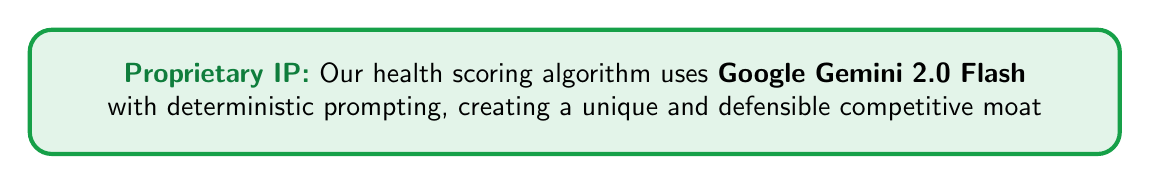
\begin{tikzpicture}
    \node[fill=successgreen!12, draw=successgreen, line width=1.5pt, rounded corners=8pt,
          inner sep=12pt, text width=13cm, align=center] {
        \textcolor{darkgreen}{\textbf{Proprietary IP:}} Our health scoring algorithm uses \textbf{Google Gemini 2.0 Flash}\\
        with deterministic prompting, creating a unique and defensible competitive moat
    };
\end{tikzpicture}
\end{center}

\subsection{Spending Analytics Dashboard}

\begin{center}
\infobox{analyticsteal}{
    \textcolor{analyticsteal}{\textbf{\large Comprehensive Financial Intelligence}}\\[12pt]
    \begin{minipage}[t]{0.48\textwidth}
        \textbf{Analytics Features:}
        \begin{itemize}[leftmargin=1.5em, itemsep=3pt]
            \item Item-level spending breakdown
            \item 16+ spending categories
            \item Store breakdown \& trends
            \item Monthly/weekly/daily tracking
            \item Budget progress monitoring
        \end{itemize}
    \end{minipage}
    \hfill
    \begin{minipage}[t]{0.48\textwidth}
        \textbf{16 Spending Categories:}\\[5pt]
        {\small Fresh Produce, Meat \& Fish, Dairy, Bakery, Beverages, Snacks \& Sweets, Frozen Foods, Pantry Staples, Health \& Beauty, Household, Baby \& Kids, Pet Supplies, Alcohol, Tobacco, Organic/Specialty, Other}
    \end{minipage}
}
\end{center}

\subsection{AI Chat Assistant (``Milo'')}

\begin{center}
\infobox{datapurple}{
    \textcolor{datapurple}{\textbf{\large Your Personal Budget \& Health Coach}}\\[12pt]
    \begin{minipage}[t]{0.55\textwidth}
        \textbf{Capabilities:}
        \begin{itemize}[leftmargin=1.5em, itemsep=3pt]
            \item Conversational AI (Gemini 2.0 Flash)
            \item Personalized spending insights
            \item Health-conscious budget coaching
            \item Transaction context (365 days)
            \item Natural language queries
        \end{itemize}
    \end{minipage}
    \hfill
    \begin{minipage}[t]{0.40\textwidth}
        \textbf{Example Interactions:}\\[5pt]
        {\small\textit{``How much did I spend on snacks last month?''}}\\[3pt]
        {\small\textit{``What's my healthiest spending week?''}}\\[3pt]
        {\small\textit{``Help me reduce my alcohol budget''}}\\[3pt]
        {\small\textit{``Compare my grocery spending to last year''}}
    \end{minipage}
}
\end{center}

\subsection{Smart Budget Management}

\begin{center}
\infobox{goldcolor}{
    \textcolor{goldcolor}{\textbf{\large Intelligent Budget Planning}}\\[12pt]
    \begin{minipage}[t]{0.48\textwidth}
        \textbf{Budget Features:}
        \begin{itemize}[leftmargin=1.5em, itemsep=3pt]
            \item Monthly budget creation
            \item Category allocations
            \item Real-time progress tracking
            \item Daily AI check-ins
            \item Instant receipt impact analysis
        \end{itemize}
    \end{minipage}
    \hfill
    \begin{minipage}[t]{0.48\textwidth}
        \textbf{Alert System:}
        \begin{itemize}[leftmargin=1.5em, itemsep=3pt]
            \item 50\% budget threshold
            \item 75\% warning alerts
            \item 90\% critical notifications
            \item Monthly AI reports with grades
            \item Savings opportunity identification
        \end{itemize}
    \end{minipage}
}
\end{center}

\section{Technical Architecture}

\begin{center}
\renewcommand{\arraystretch}{1.5}
\begin{tabular}{>{\raggedright\arraybackslash}p{4cm} >{\raggedright\arraybackslash}p{10cm}}
\toprule
\rowcolor{kbcblue!15}
\textbf{Component} & \textbf{Technology} \\
\midrule
\textbf{Frontend (iOS)} & SwiftUI 5.0+, MVVM pattern, async/await, AVFoundation \\
\rowcolor{lightbg}
\textbf{Backend} & FastAPI (Python 3.11), Uvicorn, Docker, Railway \\
\textbf{Database} & PostgreSQL with asyncpg, SQLAlchemy 2.0 \\
\rowcolor{lightbg}
\textbf{AI/ML} & Google Gemini 2.0 Flash, Veryfi API v8 \\
\textbf{Authentication} & Firebase Auth (Email, Google, Apple Sign-In) \\
\rowcolor{lightbg}
\textbf{Security} & End-to-end encryption, Keychain storage, GDPR-ready \\
\bottomrule
\end{tabular}
\end{center}

% ============================================================================
% CHAPTER 3: COMPETITOR ANALYSIS
% ============================================================================
\chapter{Comprehensive Competitor Analysis}

\section{Market Landscape Overview}

MILO operates at the intersection of three distinct markets, each with established players but \textbf{no competitor addressing all three simultaneously}:

\begin{center}
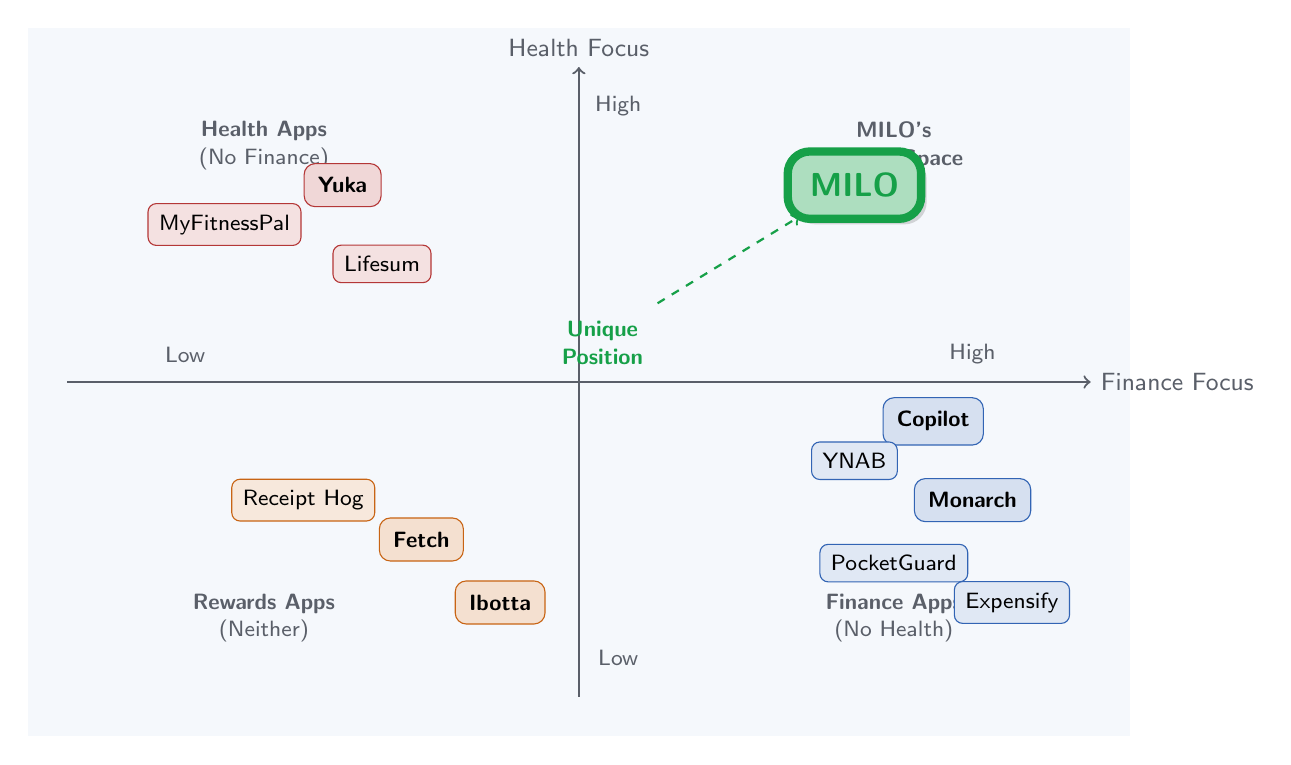
\begin{tikzpicture}
    % Background
    \fill[lightbg] (-7,-4.5) rectangle (7,4.5);

    % Axes
    \draw[->, thick, freegray] (-6.5,0) -- (6.5,0) node[right] {\small\textcolor{freegray}{Finance Focus}};
    \draw[->, thick, freegray] (0,-4) -- (0,4) node[above] {\small\textcolor{freegray}{Health Focus}};

    % Labels
    \node[freegray] at (-5,0.35) {\footnotesize Low};
    \node[freegray] at (5,0.35) {\footnotesize High};
    \node[freegray] at (0.5,3.5) {\footnotesize High};
    \node[freegray] at (0.5,-3.5) {\footnotesize Low};

    % Quadrant labels
    \node[freegray, align=center] at (-4,3) {\footnotesize\textbf{Health Apps}\\[-2pt]\footnotesize (No Finance)};
    \node[freegray, align=center] at (4,3) {\footnotesize\textbf{MILO's}\\[-2pt]\footnotesize \textbf{Unique Space}};
    \node[freegray, align=center] at (-4,-3) {\footnotesize\textbf{Rewards Apps}\\[-2pt]\footnotesize (Neither)};
    \node[freegray, align=center] at (4,-3) {\footnotesize\textbf{Finance Apps}\\[-2pt]\footnotesize (No Health)};

    % Health Apps
    \node[fill=dangerred!20, draw=dangerred, rounded corners=4pt, inner sep=5pt] at (-3,2.5) {\footnotesize\textbf{Yuka}};
    \node[fill=dangerred!15, draw=dangerred, rounded corners=3pt, inner sep=4pt] at (-4.5,2) {\footnotesize MyFitnessPal};
    \node[fill=dangerred!15, draw=dangerred, rounded corners=3pt, inner sep=4pt] at (-2.5,1.5) {\footnotesize Lifesum};

    % Rewards Apps
    \node[fill=warningorange!20, draw=warningorange, rounded corners=4pt, inner sep=5pt] at (-2,-2) {\footnotesize\textbf{Fetch}};
    \node[fill=warningorange!20, draw=warningorange, rounded corners=4pt, inner sep=5pt] at (-1,-2.8) {\footnotesize\textbf{Ibotta}};
    \node[fill=warningorange!15, draw=warningorange, rounded corners=3pt, inner sep=4pt] at (-3.5,-1.5) {\footnotesize Receipt Hog};

    % Finance Apps
    \node[fill=competitorblue!20, draw=competitorblue, rounded corners=4pt, inner sep=5pt] at (4.5,-0.5) {\footnotesize\textbf{Copilot}};
    \node[fill=competitorblue!20, draw=competitorblue, rounded corners=4pt, inner sep=5pt] at (5,-1.5) {\footnotesize\textbf{Monarch}};
    \node[fill=competitorblue!15, draw=competitorblue, rounded corners=3pt, inner sep=4pt] at (3.5,-1) {\footnotesize YNAB};
    \node[fill=competitorblue!15, draw=competitorblue, rounded corners=3pt, inner sep=4pt] at (4,-2.3) {\footnotesize PocketGuard};
    \node[fill=competitorblue!15, draw=competitorblue, rounded corners=3pt, inner sep=4pt] at (5.5,-2.8) {\footnotesize Expensify};

    % MILO - unique position with emphasis
    \node[fill=successgreen!35, draw=successgreen, line width=3pt, rounded corners=8pt, inner sep=8pt,
          drop shadow={shadow xshift=2pt, shadow yshift=-2pt, opacity=0.3}] at (3.5,2.5) {\textbf{\large\textcolor{successgreen}{MILO}}};

    % Arrow pointing to MILO's unique position
    \draw[->, thick, successgreen, dashed] (1,1) -- (2.8,2.1);
    \node[successgreen, align=center] at (0.3,0.5) {\footnotesize\textbf{Unique}\\[-2pt]\footnotesize\textbf{Position}};

\end{tikzpicture}
\end{center}

\vspace{0.3cm}

\begin{center}
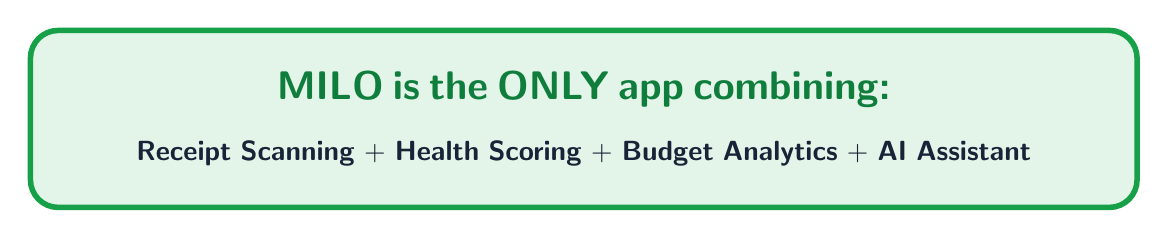
\begin{tikzpicture}
    \node[fill=successgreen!12, draw=successgreen, line width=2pt, rounded corners=10pt,
          inner sep=15pt, text width=13cm, align=center] {
        {\Large\textcolor{darkgreen}{\textbf{MILO is the ONLY app combining:}}}\\[10pt]
        \textcolor{darktext}{\textbf{Receipt Scanning} + \textbf{Health Scoring} + \textbf{Budget Analytics} + \textbf{AI Assistant}}
    };
\end{tikzpicture}
\end{center}

\newpage

\section{Budget Apps Comparison}

\subsection{YNAB (You Need A Budget)}

\begin{center}
\competitorbox{competitorblue}{YNAB --- Zero-Based Budgeting Leader}{
\begin{itemize}[leftmargin=1.2em, itemsep=2pt]
    \item \textbf{Price:} \$14.99/month or \$109/year
    \item \textbf{Users:} Millions globally
    \item \textbf{Founded:} 2004
    \item \textbf{Model:} Zero-based budgeting
    \item \textbf{Platform:} All platforms
\end{itemize}
}{
\textbf{Strengths vs MILO:}
\begin{itemize}[leftmargin=1.2em, itemsep=2pt]
    \item[\cmark] Proven methodology
    \item[\cmark] Multi-platform
    \item[\cmark] Educational resources
\end{itemize}
\textbf{Weaknesses vs MILO:}
\begin{itemize}[leftmargin=1.2em, itemsep=2pt]
    \item[\xmark] No receipt scanning
    \item[\xmark] No health features
    \item[\xmark] No item-level data
    \item[\xmark] Higher price (\$14.99 vs \$5.99)
    \item[\xmark] Steep learning curve
\end{itemize}
}{\threatlevel{successgreen}{LOW} --- Different approach entirely}
\end{center}

\subsection{Copilot Money}

\begin{center}
\competitorbox{datapurple}{Copilot --- AI-First Budgeting}{
\begin{itemize}[leftmargin=1.2em, itemsep=2pt]
    \item \textbf{Price:} \$13/month or \$95/year
    \item \textbf{Platform:} iOS, Mac, Web
    \item \textbf{Founded:} 2020
    \item \textbf{Focus:} AI-powered tracking
    \item \textbf{Integrations:} Zillow, Apple Card
\end{itemize}
}{
\textbf{Strengths vs MILO:}
\begin{itemize}[leftmargin=1.2em, itemsep=2pt]
    \item[\cmark] Beautiful UI design
    \item[\cmark] AI categorization
    \item[\cmark] Crypto support
\end{itemize}
\textbf{Weaknesses vs MILO:}
\begin{itemize}[leftmargin=1.2em, itemsep=2pt]
    \item[\xmark] No receipt scanning
    \item[\xmark] No health features
    \item[\xmark] No item-level data
    \item[\xmark] Bank-first (not receipt)
    \item[\xmark] Higher price (\$13 vs \$5.99)
    \item[\xmark] Apple-only
\end{itemize}
}{\threatlevel{warningorange}{MEDIUM} --- Similar AI approach, different data}
\end{center}

\subsection{Monarch Money}

\begin{center}
\competitorbox{competitorblue}{Monarch Money --- Household Finance Leader}{
\begin{itemize}[leftmargin=1.2em, itemsep=2pt]
    \item \textbf{Price:} \$14.99/month or \$99.99/year
    \item \textbf{Users:} Growing rapidly (2,000\% growth)
    \item \textbf{Funding:} \$75M raised
    \item \textbf{Recognition:} WSJ ``Best Budgeting App''
    \item \textbf{Platform:} iOS, Android, Web
\end{itemize}
}{
\textbf{Strengths vs MILO:}
\begin{itemize}[leftmargin=1.2em, itemsep=2pt]
    \item[\cmark] Multi-user/household
    \item[\cmark] Investment tracking
    \item[\cmark] Cash flow forecasting
    \item[\cmark] Mint replacement positioning
\end{itemize}
\textbf{Weaknesses vs MILO:}
\begin{itemize}[leftmargin=1.2em, itemsep=2pt]
    \item[\xmark] No receipt scanning
    \item[\xmark] No health features
    \item[\xmark] No item-level granularity
    \item[\xmark] Higher price (\$14.99 vs \$5.99)
    \item[\xmark] Bank-centric approach
\end{itemize}
}{\threatlevel{warningorange}{MEDIUM} --- Could be complementary}
\end{center}

\subsection{PocketGuard}

\begin{center}
\competitorbox{miloaccent}{PocketGuard --- ``In My Pocket'' Focus}{
\begin{itemize}[leftmargin=1.2em, itemsep=2pt]
    \item \textbf{Price:} \$12.99/month or \$74.99/year
    \item \textbf{Trial:} 7-day free trial
    \item \textbf{Focus:} Disposable income tracking
    \item \textbf{Features:} Auto-detects subscriptions
    \item \textbf{Platform:} iOS, Android, Web, Apple Watch
\end{itemize}
}{
\textbf{Strengths vs MILO:}
\begin{itemize}[leftmargin=1.2em, itemsep=2pt]
    \item[\cmark] Simple ``In My Pocket'' concept
    \item[\cmark] Subscription manager
    \item[\cmark] Bill negotiation
\end{itemize}
\textbf{Weaknesses vs MILO:}
\begin{itemize}[leftmargin=1.2em, itemsep=2pt]
    \item[\xmark] No receipt scanning
    \item[\xmark] No health features
    \item[\xmark] No item-level data
    \item[\xmark] Higher price (\$12.99 vs \$5.99)
    \item[\xmark] ``Janky'' UI per reviews
\end{itemize}
}{\threatlevel{successgreen}{LOW} --- Different value proposition}
\end{center}

\newpage

\section{Receipt Scanning Apps Comparison}

\subsection{Fetch Rewards}

\begin{center}
\competitorbox{warningorange}{Fetch Rewards --- Largest Receipt App}{
\begin{itemize}[leftmargin=1.2em, itemsep=2pt]
    \item \textbf{Users:} 17M+ MAU
    \item \textbf{Valuation:} \$2.5 billion
    \item \textbf{Daily Receipts:} 1M+ processed
    \item \textbf{Price:} Free (data monetization)
    \item \textbf{Model:} Scan any receipt for points
\end{itemize}
}{
\textbf{Strengths vs MILO:}
\begin{itemize}[leftmargin=1.2em, itemsep=2pt]
    \item[\cmark] Massive user base
    \item[\cmark] Free for users
    \item[\cmark] Simple value prop
    \item[\cmark] Strong partnerships
\end{itemize}
\textbf{Weaknesses vs MILO:}
\begin{itemize}[leftmargin=1.2em, itemsep=2pt]
    \item[\xmark] No health features
    \item[\xmark] No spending analytics
    \item[\xmark] Privacy concerns (data selling)
    \item[\xmark] Users are the product
    \item[\xmark] No AI assistant
\end{itemize}
}{\threatlevel{warningorange}{MEDIUM} --- Different value proposition}
\end{center}

\subsection{Ibotta}

\begin{center}
\competitorbox{warningorange}{Ibotta --- Cashback Leader}{
\begin{itemize}[leftmargin=1.2em, itemsep=2pt]
    \item \textbf{Users:} 40M+ total
    \item \textbf{Valuation:} \$3B+ (IPO filed 2024)
    \item \textbf{Partners:} 180+ retail partnerships
    \item \textbf{Price:} Free (cashback model)
    \item \textbf{Model:} Pre-select offers, upload receipt
\end{itemize}
}{
\textbf{Strengths vs MILO:}
\begin{itemize}[leftmargin=1.2em, itemsep=2pt]
    \item[\cmark] Real cash back
    \item[\cmark] Strong retail partnerships
    \item[\cmark] IPO trajectory
\end{itemize}
\textbf{Weaknesses vs MILO:}
\begin{itemize}[leftmargin=1.2em, itemsep=2pt]
    \item[\xmark] No health features
    \item[\xmark] No spending analytics
    \item[\xmark] Requires pre-selecting offers
    \item[\xmark] Commoditized model
    \item[\xmark] No AI insights
\end{itemize}
}{\threatlevel{warningorange}{MEDIUM} --- Users familiar with scanning}
\end{center}

\section{Health Apps Comparison}

\subsection{Yuka --- Strategic Opportunity}

\begin{center}
\competitorbox{successgreen}{Yuka --- Health Scanning Leader (Potential Partner)}{
\begin{itemize}[leftmargin=1.2em, itemsep=2pt]
    \item \textbf{Users:} 80M globally, 20M+ in US
    \item \textbf{Revenue:} \$20.3M (2023)
    \item \textbf{Growth:} 25,000 new US users/day
    \item \textbf{Database:} 4M food + 2M cosmetics
    \item \textbf{Model:} Premium subscriptions (\$10/mo)
\end{itemize}
}{
\textbf{Why LOW Threat:}
\begin{itemize}[leftmargin=1.2em, itemsep=2pt]
    \item[\xmark] No receipt scanning
    \item[\xmark] No spending analytics
    \item[\xmark] No purchase history
    \item[\xmark] Point-of-decision only
    \item[\xmark] Different use case
\end{itemize}
\textbf{Opportunity:}\\[5pt]
\textcolor{darkgreen}{\textbf{Yuka users = Ideal MILO targets}}\\
Health-conscious consumers who would value post-purchase insights.
}{\threatlevel{successgreen}{LOW} --- Complementary, not competitive}
\end{center}

\vspace{0.3cm}

\begin{center}
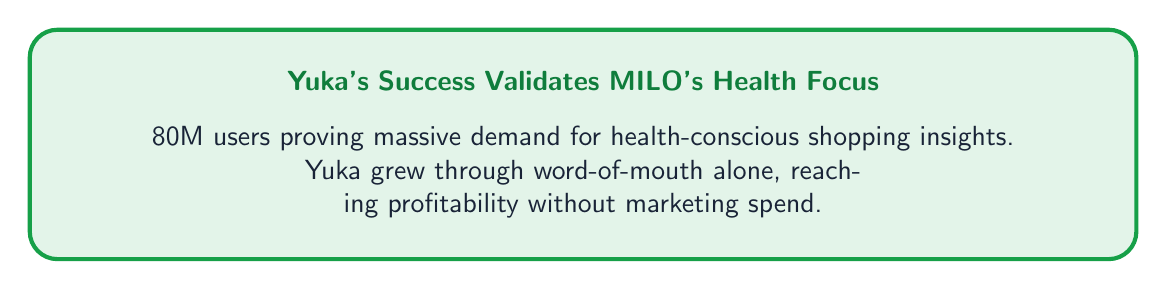
\begin{tikzpicture}
    \node[fill=successgreen!12, draw=successgreen, line width=1.5pt, rounded corners=10pt,
          inner sep=15pt, text width=13cm, align=center] {
        \textcolor{darkgreen}{\textbf{Yuka's Success Validates MILO's Health Focus}}\\[8pt]
        \textcolor{darktext}{80M users proving massive demand for health-conscious shopping insights.}\\
        \textcolor{darktext}{Yuka grew through word-of-mouth alone, reaching profitability without marketing spend.}
    };
\end{tikzpicture}
\end{center}

\newpage

\section{Comprehensive Feature Comparison}

\begin{center}
\renewcommand{\arraystretch}{1.5}
\begin{tabular}{>{\raggedright\arraybackslash}p{3.5cm} >{\centering\arraybackslash}p{1.5cm} >{\centering\arraybackslash}p{1.5cm} >{\centering\arraybackslash}p{1.5cm} >{\centering\arraybackslash}p{1.5cm} >{\centering\arraybackslash}p{1.5cm} >{\centering\arraybackslash}p{1.5cm}}
\toprule
\rowcolor{kbcblue!15}
\textbf{Feature} & \textbf{MILO} & \textbf{YNAB} & \textbf{Copilot} & \textbf{Monarch} & \textbf{Fetch} & \textbf{Yuka} \\
\midrule
Receipt Scanning & \cmark & \xmark & \xmark & \xmark & \cmark & \xmark \\
\rowcolor{lightbg}
Health Scores & \cmark & \xmark & \xmark & \xmark & \xmark & \cmark \\
Spending Analytics & \cmark & \cmark & \cmark & \cmark & \xmark & \xmark \\
\rowcolor{lightbg}
AI Categorization & \cmark & \xmark & \cmark & Limited & Limited & N/A \\
AI Chat Assistant & \cmark & \xmark & \cmark & \xmark & \xmark & \xmark \\
\rowcolor{lightbg}
Item-Level Data & \cmark & \xmark & \xmark & \xmark & \xmark & N/A \\
Budget Tracking & \cmark & \cmark & \cmark & \cmark & \xmark & \xmark \\
\rowcolor{lightbg}
Bank Connections & \xmark & \cmark & \cmark & \cmark & \xmark & N/A \\
\midrule
\rowcolor{successgreen!10}
\textbf{Entry Price} & \textcolor{successgreen}{\textbf{\$5.99}} & \$14.99 & \$13 & \$14.99 & Free* & Free \\
\bottomrule
\end{tabular}
\end{center}

{\small *Free but users' data is monetized to brands}

\vspace{0.5cm}

\section{Pricing Comparison}

\begin{center}
\renewcommand{\arraystretch}{1.5}
\begin{tabular}{>{\raggedright\arraybackslash}p{3.5cm} >{\centering\arraybackslash}p{2.5cm} >{\centering\arraybackslash}p{2.5cm} >{\centering\arraybackslash}p{2.5cm} >{\centering\arraybackslash}p{2.5cm}}
\toprule
\rowcolor{kbcblue!15}
\textbf{App} & \textbf{Monthly} & \textbf{Annual} & \textbf{Full Features} & \textbf{Health} \\
\midrule
\rowcolor{successgreen!15}
\textcolor{kbcblue}{\textbf{MILO Gold}} & \textcolor{successgreen}{\textbf{\$5.99}} & \textcolor{successgreen}{\textbf{\$54.99}} & \cmark\ All tiers & \cmark \\
YNAB & \$14.99 & \$109 & \cmark & \xmark \\
\rowcolor{lightbg}
Copilot & \$13 & \$95 & \cmark & \xmark \\
Monarch & \$14.99 & \$99.99 & \cmark & \xmark \\
\rowcolor{lightbg}
PocketGuard & \$12.99 & \$74.99 & \cmark & \xmark \\
Yuka Premium & $\sim$\$10 & $\sim$\$30 & \cmark & \cmark \\
\rowcolor{lightbg}
Fetch/Ibotta & Free* & Free* & N/A & \xmark \\
\bottomrule
\end{tabular}
\end{center}

\vspace{0.3cm}

\begin{center}
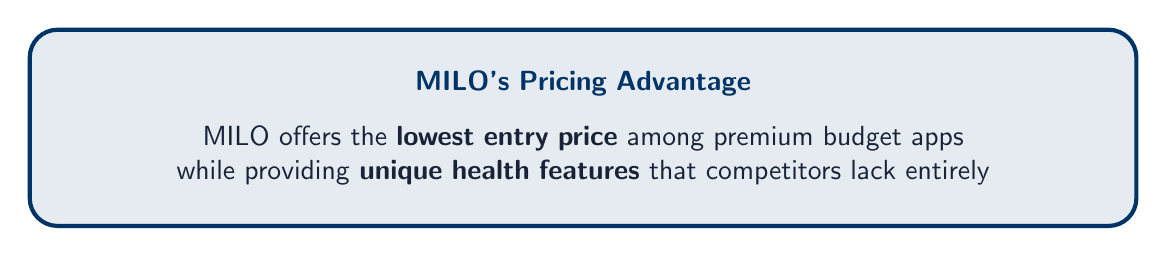
\begin{tikzpicture}
    \node[fill=kbcblue!10, draw=kbcblue, line width=1.5pt, rounded corners=10pt,
          inner sep=15pt, text width=13cm, align=center] {
        \textcolor{kbcblue}{\textbf{MILO's Pricing Advantage}}\\[8pt]
        \textcolor{darktext}{MILO offers the \textbf{lowest entry price} among premium budget apps}\\
        \textcolor{darktext}{while providing \textbf{unique health features} that competitors lack entirely}
    };
\end{tikzpicture}
\end{center}

\newpage

\section{MILO's Competitive Advantages}

\begin{center}
\infobox{kbcblue}{
    {\Large\textcolor{kbcblue}{\textbf{Why MILO Wins}}}\\[15pt]

    \begin{minipage}[t]{0.48\textwidth}
        \textbf{\textcolor{successgreen}{1. Unique Market Position}}
        \begin{itemize}[leftmargin=1.5em, itemsep=4pt]
            \item Only app combining receipts + health + budgeting
            \item Item-level granularity (not just transactions)
            \item Consumer-first (not B2B repackaged)
            \item Privacy-respecting subscription model
        \end{itemize}

        \vspace{12pt}
        \textbf{\textcolor{successgreen}{2. AI-Native Architecture}}
        \begin{itemize}[leftmargin=1.5em, itemsep=4pt]
            \item Built for AI from day one
            \item Intelligent categorization (16+ categories)
            \item Proprietary health scoring (0--5 scale)
            \item Conversational AI assistant
        \end{itemize}
    \end{minipage}
    \hfill
    \begin{minipage}[t]{0.48\textwidth}
        \textbf{\textcolor{successgreen}{3. Aggressive Pricing}}
        \begin{itemize}[leftmargin=1.5em, itemsep=4pt]
            \item \$5.99/mo entry --- 50\% below competitors
            \item Full features at every tier
            \item Volume-based, not feature-gated
            \item 17\% annual discount
        \end{itemize}

        \vspace{12pt}
        \textbf{\textcolor{successgreen}{4. Defensible Moat}}
        \begin{itemize}[leftmargin=1.5em, itemsep=4pt]
            \item Proprietary health scoring IP
            \item Data network effects
            \item Privacy positioning (GDPR as feature)
            \item Switching costs (historical data)
        \end{itemize}
    \end{minipage}
}
\end{center}

\vspace{0.5cm}

\section{Competitive Threat Assessment}

\begin{center}
\renewcommand{\arraystretch}{1.5}
\begin{tabular}{>{\raggedright\arraybackslash}p{3cm} >{\centering\arraybackslash}p{2cm} >{\centering\arraybackslash}p{2cm} >{\centering\arraybackslash}p{2cm} >{\raggedright\arraybackslash}p{4.5cm}}
\toprule
\rowcolor{kbcblue!15}
\textbf{Competitor} & \textbf{Market Overlap} & \textbf{Feature Overlap} & \textbf{Threat} & \textbf{MILO's Defensive Moat} \\
\midrule
\rowcolor{warningorange!8}
Fetch Rewards & High & Low & \threatlevel{warningorange}{MEDIUM} & Health features, analytics, privacy \\
Ibotta & High & Low & \threatlevel{warningorange}{MEDIUM} & Health features, analytics, privacy \\
\rowcolor{warningorange!8}
Copilot & Medium & Medium & \threatlevel{warningorange}{MEDIUM} & Receipt data, health scoring, price \\
Monarch & Medium & Low & \threatlevel{warningorange}{MEDIUM} & Receipt data, health, item-level \\
\rowcolor{successgreen!8}
YNAB & Low & Low & \threatlevel{successgreen}{LOW} & Completely different methodology \\
PocketGuard & Low & Low & \threatlevel{successgreen}{LOW} & Health features, AI assistant \\
\rowcolor{successgreen!8}
Yuka & Medium & Low & \threatlevel{successgreen}{LOW} & Spending analytics, receipts \\
\bottomrule
\end{tabular}
\end{center}

\vspace{0.3cm}

\begin{center}
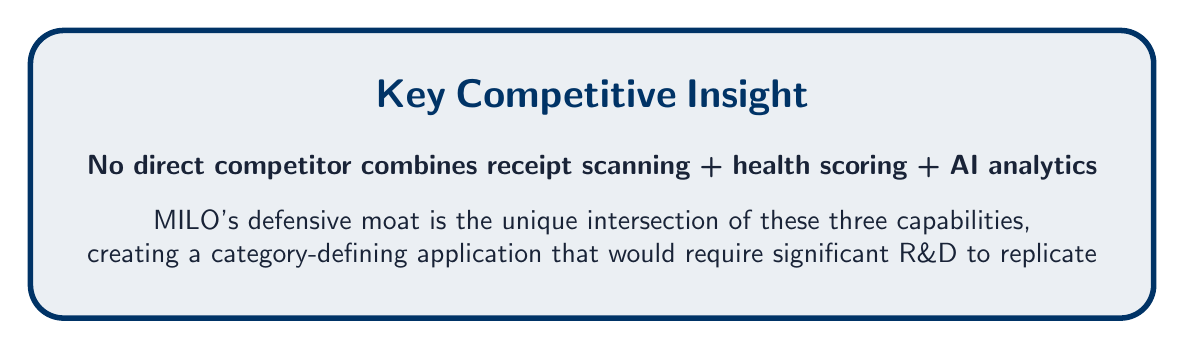
\begin{tikzpicture}
    \node[fill=kbcblue!8, draw=kbcblue, line width=2pt, rounded corners=12pt,
          inner sep=18pt, text width=13cm, align=center] {
        {\Large\textcolor{kbcblue}{\textbf{Key Competitive Insight}}}\\[12pt]
        \textcolor{darktext}{\textbf{No direct competitor combines receipt scanning + health scoring + AI analytics}}\\[8pt]
        \textcolor{darktext}{MILO's defensive moat is the unique intersection of these three capabilities,}\\
        \textcolor{darktext}{creating a category-defining application that would require significant R\&D to replicate}
    };
\end{tikzpicture}
\end{center}

% ============================================================================
% CHAPTER 4: MARKET OPPORTUNITY
% ============================================================================
\chapter{Market Opportunity}

\section{Total Addressable Market: \$21.7B+}

MILO operates at the intersection of three massive, growing markets:

\begin{center}
\renewcommand{\arraystretch}{1.5}
\begin{tabular}{>{\raggedright\arraybackslash}p{5cm} >{\centering\arraybackslash}p{2.5cm} >{\centering\arraybackslash}p{2.5cm} >{\centering\arraybackslash}p{2.5cm}}
\toprule
\rowcolor{kbcblue!15}
\textbf{Market Segment} & \textbf{2025} & \textbf{2030} & \textbf{CAGR} \\
\midrule
Receipt Scanner Apps & \$2.5B & \$5.1B & 11.1\% \\
\rowcolor{lightbg}
Personal Finance Apps & \$7.2B & \$14.4B & 12.3\% \\
Consumer Data Monetization & \$12.0B & \$26.5B & 22.0\% \\
\midrule
\rowcolor{successgreen!10}
\textbf{Combined TAM} & \textbf{\$21.7B} & \textbf{\$46.0B} & \textbf{15.1\%} \\
\bottomrule
\end{tabular}
\end{center}

\vspace{0.3cm}

\begin{center}
\sourcebox{Growth Market Reports 2024, Fortune Business Insights 2025, Global Wellness Institute 2025}
\end{center}

\section{Target Market Segments}

\begin{center}
\renewcommand{\arraystretch}{1.5}
\begin{tabular}{>{\raggedright\arraybackslash}p{4cm} >{\centering\arraybackslash}p{2cm} >{\centering\arraybackslash}p{3cm} >{\centering\arraybackslash}p{2.5cm} >{\centering\arraybackslash}p{2cm}}
\toprule
\rowcolor{kbcblue!15}
\textbf{Segment} & \textbf{Size (US)} & \textbf{Demographics} & \textbf{Income} & \textbf{WTP} \\
\midrule
\rowcolor{healthgreen!8}
Health Optimizers & 22M users & Ages 25-40 & \$60K-150K & \$6-10/mo \\
Ex-Mint Users & 6M displaced & Ages 28-45 & \$50K-120K & \$10-20/mo \\
\rowcolor{healthgreen!8}
Wellness Families & 15M & Ages 30-50 & \$80K-200K & \$15-20/mo \\
GLP-1 Users & 15M+ & Ages 25-55 & \$75K-200K & \$15-20/mo \\
\bottomrule
\end{tabular}
\end{center}

\section{Why Now: The Perfect Storm}

\textbf{Consumer Behavior Shift:}
\begin{itemize}[leftmargin=2em, itemsep=4pt]
    \item 85\% of consumers actively check nutrition labels (IFIC 2024)
    \item 16\% of US households now use GLP-1 medications---creating massive health awareness
    \item Mint.com shut down March 2024, leaving 3.6M users seeking alternatives
    \item 94\% of Yuka users stopped buying products flagged as unhealthy (Yuka Impact Study 2024)
\end{itemize}

\textbf{Technology Inflection Point:}
\begin{itemize}[leftmargin=2em, itemsep=4pt]
    \item AI costs dropped 95\%+ in 24 months---making our product economically viable
    \item OCR accuracy hit 99\%+---receipt scanning finally works flawlessly
    \item Mobile-first consumers expect instant, passive tracking
\end{itemize}

\textbf{Market Dynamics:}
\begin{itemize}[leftmargin=2em, itemsep=4pt]
    \item Mobile rewards industry: \$25 billion market
    \item 72\% of consumers choose brands with strong rewards programs
    \item Privacy-compliant data commands 3x premium over scraped data
\end{itemize}

% ============================================================================
% CHAPTER 5: BUSINESS MODEL
% ============================================================================
\chapter{Business Model \& Revenue}

\section{Three-Pillar Revenue Architecture}

\begin{center}
    \revenuestream{appstoreblue}{B2C Subscriptions}{\$580K}{24-35\% of revenue}
    \hspace{0.3cm}
    \revenuestream{datapurple}{B2B Data Licensing}{\$1.56M}{52-66\% of revenue}
    \hspace{0.3cm}
    \revenuestream{analyticsteal}{Analytics Reports}{\$250K}{10-13\% of revenue}
\end{center}

\vspace{0.5cm}

\section{Subscription Pricing}

\begin{center}
    \tierbox{silvercolor}{SILVER}{25}{\$5.99/mo}{\$54.99/year}
    \hspace{0.2cm}
    \tierbox{goldcolor}{GOLD}{40}{\$6.49/mo}{\$59.99/year}
    \hspace{0.2cm}
    \tierbox{platinumcolor}{PLATINUM}{150}{\$17.49/mo}{\$149.99/year}
\end{center}

\vspace{0.5cm}

\begin{center}
\renewcommand{\arraystretch}{1.5}
\begin{tabular}{>{\raggedright\arraybackslash}p{2.5cm} >{\centering\arraybackslash}p{2cm} >{\centering\arraybackslash}p{2cm} >{\centering\arraybackslash}p{2.5cm} >{\centering\arraybackslash}p{2.5cm} >{\centering\arraybackslash}p{2.5cm}}
\toprule
\rowcolor{kbcblue!15}
\textbf{Tier} & \textbf{Receipts} & \textbf{Monthly} & \textbf{Annual} & \textbf{Gross LTV} & \textbf{LTV:CAC} \\
\midrule
\rowcolor{silvercolor!10}
\textbf{Silver} & 25/mo & \$5.99 & \$54.99 & \$90.86 & 5.3:1 \\
\rowcolor{goldcolor!10}
\textbf{Gold} & 40/mo & \$6.49 & \$59.99 & \$98.35 & 5.8:1 \\
\rowcolor{platinumcolor!10}
\textbf{Platinum} & 150/mo & \$17.49 & \$149.99 & \$314.82 & 18.5:1 \\
\midrule
\rowcolor{successgreen!10}
\textbf{Blended} & -- & -- & -- & \textbf{\$110+} & \textbf{6:1+} \\
\bottomrule
\end{tabular}
\end{center}

\section{B2B Data Monetization}

\begin{center}
\infobox{datapurple}{
    \textcolor{datapurple}{\textbf{\large Premium Consumer Purchase Intelligence}}\\[12pt]
    MILO's data is differentiated by \textbf{item-level granularity} (10-50 data points per receipt vs. 1-3 for competitors) and \textbf{proprietary health scoring}. All data is explicitly consented, GDPR-compliant, and commands premium pricing.\\[12pt]
    \begin{minipage}[t]{0.48\textwidth}
        \textbf{Revenue Streams:}
        \begin{itemize}[leftmargin=1.5em, itemsep=3pt]
            \item DaaS: \$30-75 per panelist/year
            \item Syndicated Reports: \$2.5K-50K each
            \item Custom Research: \$5K-100K+ per study
            \item Analytics Platform: \$5K-50K/year
        \end{itemize}
    \end{minipage}
    \hfill
    \begin{minipage}[t]{0.48\textwidth}
        \textbf{Target Enterprise Buyers:}
        \begin{itemize}[leftmargin=1.5em, itemsep=3pt]
            \item CPG brands (Nestl\'{e}, P\&G, Unilever)
            \item Retailers (Kroger, Whole Foods)
            \item Health/wellness companies
            \item Market research firms
        \end{itemize}
    \end{minipage}
}
\end{center}

\section{Financial Projections (Conservative Case)}

\begin{center}
\renewcommand{\arraystretch}{1.5}
\begin{tabular}{>{\raggedright\arraybackslash}p{5cm} >{\centering\arraybackslash}p{3cm} >{\centering\arraybackslash}p{3cm} >{\centering\arraybackslash}p{3cm}}
\toprule
\rowcolor{kbcblue!15}
\textbf{Metric} & \textbf{Year 1} & \textbf{Year 2} & \textbf{Year 3} \\
\midrule
\textbf{Monthly Active Users} & 3,500 & 9,000 & 25,000 \\
\rowcolor{lightbg}
\textbf{Total Revenue} & \$228K & \$1.1M & \$2.4M \\
\quad B2C Subscriptions & \$228K & \$660K & \$580K \\
\rowcolor{lightbg}
\quad B2B Data Licensing & \$0 & \$420K & \$1.56M \\
\quad Analytics Reports & \$0 & \$50K & \$250K \\
\midrule
\textbf{Total Operating Costs} & \$300K & \$700K & \$1.0M \\
\rowcolor{lightbg}
\textbf{Operating Profit/(Loss)} & \textbf{(\$72K)} & \textbf{\$418K} & \textbf{\$1.39M} \\
\rowcolor{successgreen!10}
\textbf{Operating Margin} & -31.6\% & 38.0\% & \textbf{58.0\%} \\
\bottomrule
\end{tabular}
\end{center}

\vspace{0.3cm}

\begin{center}
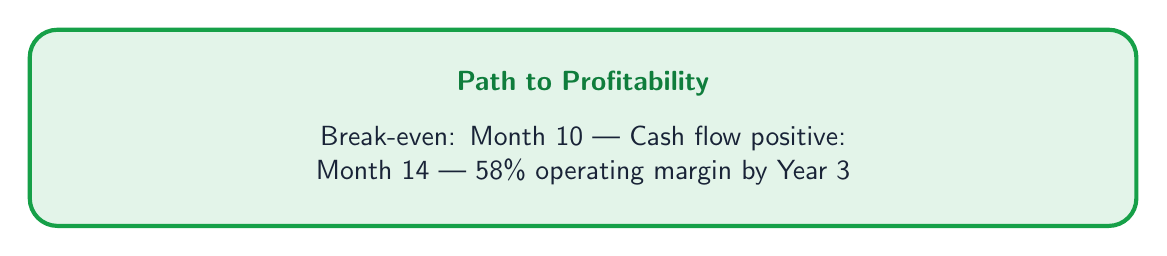
\begin{tikzpicture}
    \node[fill=successgreen!12, draw=successgreen, line width=1.5pt, rounded corners=10pt,
          inner sep=15pt, text width=13cm, align=center] {
        \textcolor{darkgreen}{\textbf{Path to Profitability}}\\[8pt]
        \textcolor{darktext}{Break-even: Month 10 | Cash flow positive: Month 14 | 58\% operating margin by Year 3}
    };
\end{tikzpicture}
\end{center}

% ============================================================================
% CHAPTER 6: RISK ANALYSIS
% ============================================================================
\chapter{Risk Analysis \& Mitigation}

\section{Key Risks \& Mitigations}

\begin{center}
\infobox{warningorange}{
    \textcolor{warningorange}{\textbf{\Large Critical Risks}}\\[12pt]
    \begin{minipage}[t]{0.48\textwidth}
        \textbf{\textcolor{dangerred}{1. GDPR Non-Compliance (Critical)}}
        \begin{itemize}[leftmargin=1.5em, itemsep=3pt]
            \item \textbf{Impact:} Cannot launch in EU
            \item \textbf{Status:} 25/100 readiness
            \item \textbf{Cost:} \euro 75K-115K
            \item \textbf{Mitigation:} 12-week compliance roadmap
        \end{itemize}

        \vspace{8pt}
        \textbf{\textcolor{dangerred}{2. Insufficient Funding (Critical)}}
        \begin{itemize}[leftmargin=1.5em, itemsep=3pt]
            \item \textbf{Impact:} Operations cease
            \item \textbf{Mitigation:} Conservative projections
            \item \textbf{Backup:} Phased development approach
        \end{itemize}
    \end{minipage}
    \hfill
    \begin{minipage}[t]{0.48\textwidth}
        \textbf{\textcolor{warningorange}{3. User Data Consent Below 60\% (High)}}
        \begin{itemize}[leftmargin=1.5em, itemsep=3pt]
            \item \textbf{Impact:} \$1M revenue loss per 10\% decline
            \item \textbf{Mitigation:} Clear value exchange, gamification
        \end{itemize}

        \vspace{8pt}
        \textbf{\textcolor{warningorange}{4. Veryfi API Cost Increase (High)}}
        \begin{itemize}[leftmargin=1.5em, itemsep=3pt]
            \item \textbf{Impact:} 91\% of variable costs
            \item \textbf{Mitigation:} Volume contracts, alternative OCR
        \end{itemize}

        \vspace{8pt}
        \textbf{\textcolor{successgreen}{5. Competition (Medium)}}
        \begin{itemize}[leftmargin=1.5em, itemsep=3pt]
            \item \textbf{Impact:} Market share erosion
            \item \textbf{Mitigation:} First-mover advantage, health moat
        \end{itemize}
    \end{minipage}
}
\end{center}

\section{Scenario Analysis}

\begin{center}
\renewcommand{\arraystretch}{1.5}
\begin{tabular}{>{\raggedright\arraybackslash}p{3.5cm} >{\centering\arraybackslash}p{2.5cm} >{\centering\arraybackslash}p{2.5cm} >{\centering\arraybackslash}p{2.5cm} >{\centering\arraybackslash}p{2cm}}
\toprule
\rowcolor{kbcblue!15}
\textbf{Scenario} & \textbf{Y3 Revenue} & \textbf{Y3 Profit} & \textbf{Valuation (8x)} & \textbf{Probability} \\
\midrule
\rowcolor{dangerred!10}
Bear Case & \$1.2M & \$100K & \$9.6M & 20\% \\
\rowcolor{lightbg}
\textbf{Base Case} & \textbf{\$2.4M} & \textbf{\$1.39M} & \textbf{\$19.2M} & 60\% \\
\rowcolor{successgreen!10}
Bull Case & \$4.5M & \$2.5M & \$36M & 20\% \\
\bottomrule
\end{tabular}
\end{center}

% ============================================================================
% CHAPTER 7: WHY KBC START IT
% ============================================================================
\chapter{Why KBC Start It}

\section{Strategic Fit with KBC}

\begin{center}
\infobox{kbcblue}{
    \textcolor{kbcblue}{\textbf{\large Why MILO is Perfect for KBC Start It}}\\[12pt]
    \begin{minipage}[t]{0.48\textwidth}
        \textbf{Alignment with KBC's Vision:}
        \begin{itemize}[leftmargin=1.5em, itemsep=4pt]
            \item FinTech innovation in personal finance
            \item Health \& wellness integration
            \item AI-powered consumer solutions
            \item European privacy-first approach
            \item Data-driven insights platform
        \end{itemize}
    \end{minipage}
    \hfill
    \begin{minipage}[t]{0.48\textwidth}
        \textbf{What MILO Needs from KBC:}
        \begin{itemize}[leftmargin=1.5em, itemsep=4pt]
            \item Seed capital (\$500K-\$750K)
            \item Banking \& FinTech expertise
            \item European market access
            \item Regulatory guidance (GDPR)
            \item Strategic partnerships
        \end{itemize}
    \end{minipage}
}
\end{center}

\section{Investment Return Potential}

\begin{center}
\renewcommand{\arraystretch}{1.5}
\begin{tabular}{>{\raggedright\arraybackslash}p{4cm} >{\centering\arraybackslash}p{3cm} >{\centering\arraybackslash}p{3cm} >{\centering\arraybackslash}p{3cm}}
\toprule
\rowcolor{kbcblue!15}
\textbf{Scenario} & \textbf{Valuation (Y3)} & \textbf{Multiple} & \textbf{Return on \$500K} \\
\midrule
\rowcolor{lightbg}
Conservative & \$9.6M & 5x & 3-4x \\
\textbf{Base Case} & \textbf{\$19.2M} & \textbf{8x} & \textbf{8-10x} \\
\rowcolor{successgreen!10}
Optimistic & \$36M & 12x & 15-18x \\
\bottomrule
\end{tabular}
\end{center}

\section{The Ask}

\begin{center}
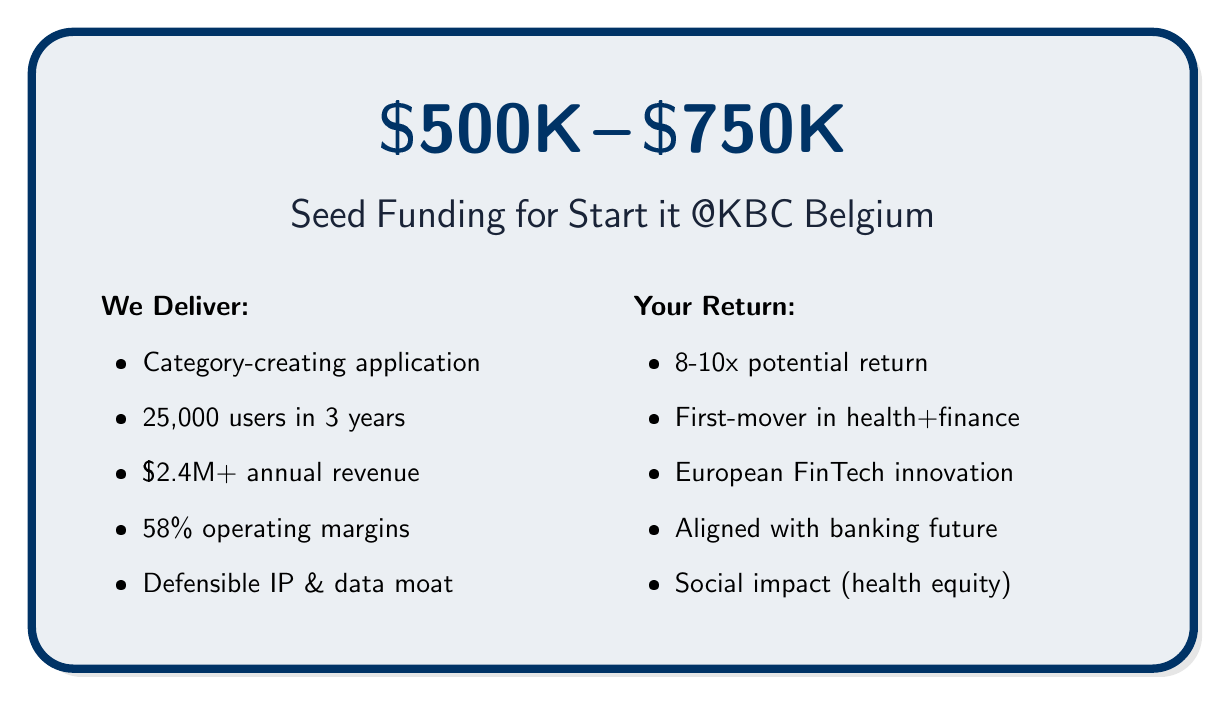
\begin{tikzpicture}
    \node[fill=kbcblue!8, draw=kbcblue, line width=3pt, rounded corners=15pt,
          inner sep=25pt, text width=13cm, align=center,
          drop shadow={shadow xshift=3pt, shadow yshift=-3pt, opacity=0.2}] {
        {\Huge\textcolor{kbcblue}{\textbf{\$500K -- \$750K}}}\\[15pt]
        {\Large\textcolor{darktext}{Seed Funding for Start it @KBC Belgium}}\\[20pt]

        \begin{minipage}[t]{0.48\textwidth}
            \textbf{We Deliver:}
            \begin{itemize}[leftmargin=1.5em, itemsep=4pt]
                \item Category-creating application
                \item 25,000 users in 3 years
                \item \$2.4M+ annual revenue
                \item 58\% operating margins
                \item Defensible IP \& data moat
            \end{itemize}
        \end{minipage}
        \hfill
        \begin{minipage}[t]{0.48\textwidth}
            \textbf{Your Return:}
            \begin{itemize}[leftmargin=1.5em, itemsep=4pt]
                \item 8-10x potential return
                \item First-mover in health+finance
                \item European FinTech innovation
                \item Aligned with banking future
                \item Social impact (health equity)
            \end{itemize}
        \end{minipage}
    };
\end{tikzpicture}
\end{center}

\vspace{1cm}

\begin{center}
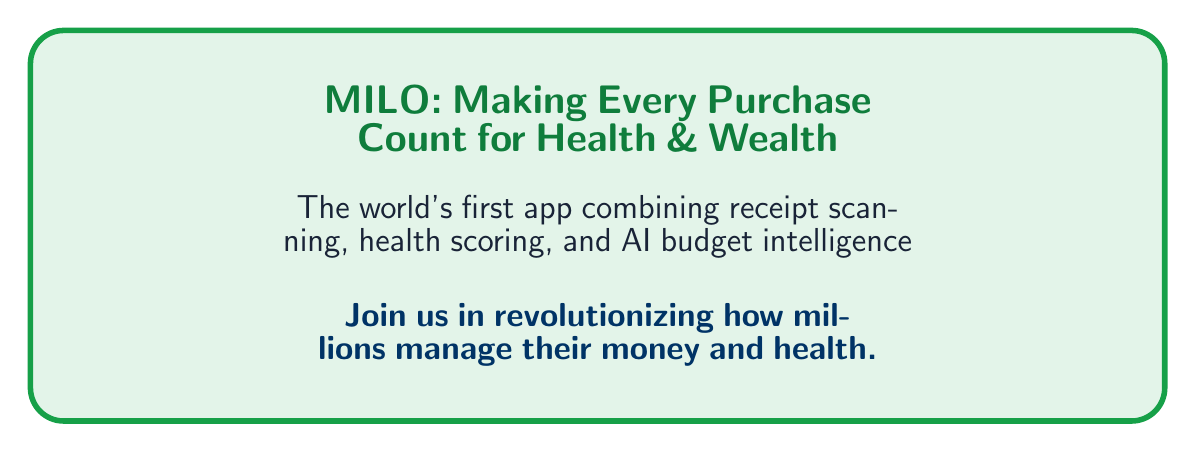
\begin{tikzpicture}
    \node[fill=successgreen!12, draw=successgreen, line width=2pt, rounded corners=12pt,
          inner sep=20pt, text width=13cm, align=center] {
        {\Large\textcolor{darkgreen}{\textbf{MILO: Making Every Purchase Count for Health \& Wealth}}}\\[12pt]
        {\large\textcolor{darktext}{The world's first app combining receipt scanning, health scoring, and AI budget intelligence}}\\[15pt]
        {\large\textcolor{kbcblue}{\textbf{Join us in revolutionizing how millions manage their money and health.}}}
    };
\end{tikzpicture}
\end{center}

\vspace{1.5cm}

% ============================================================================
% FOOTER
% ============================================================================
\begin{center}
    \textcolor{freegray}{\rule{13cm}{0.5pt}}\\[0.5cm]
    \textcolor{freegray}{\textbf{DeepmAInd B.V.} | Belgium | Confidential}\\[0.3cm]
    \textcolor{freegray}{Version 5.0 | January 2026}\\[0.3cm]
    \textcolor{kbcblue}{\textbf{Application for Start it @KBC Belgium}}
\end{center}

\end{document}
